%%% タイトル sympo2303
\documentclass[landscape,10pt]{ujarticle}
\special{papersize=\the\paperwidth,\the\paperheight}
\usepackage{ketpic,ketlayer}
\usepackage{ketslide}
\usepackage{amsmath,amssymb}
\usepackage{bm,enumerate}
\usepackage[dvipdfmx]{graphicx}
\usepackage{color}
\definecolor{slidecolora}{cmyk}{0.98,0.13,0,0.43}
\definecolor{slidecolorb}{cmyk}{0.2,0,0,0}
\definecolor{slidecolorc}{cmyk}{0.2,0,0,0}
\definecolor{slidecolord}{cmyk}{0.2,0,0,0}
\definecolor{slidecolore}{cmyk}{0,0,0,0.5}
\definecolor{slidecolorf}{cmyk}{0,0,0,0.5}
\definecolor{slidecolori}{cmyk}{0.98,0.13,0,0.43}
\def\setthin#1{\def\thin{#1}}
\setthin{0}
\newcommand{\slidepage}[1][s]{%
\setcounter{ketpicctra}{18}%
\if#1m \setcounter{ketpicctra}{1}\fi
\hypersetup{linkcolor=black}%

\begin{layer}{118}{0}
\putnotee{122}{-\theketpicctra.05}{\small\thepage/\pageref{pageend}}
\end{layer}\hypersetup{linkcolor=blue}

}
\usepackage[dvipdfmx,colorlinks=true,linkcolor=blue,filecolor=blue]{hyperref}
\newcommand{\hiduke}{0304}
\newcommand{\hako}[2][1]{\fbox{\raisebox{#1mm}{\mbox{}}\raisebox{-#1mm}{\mbox{}}\,\phantom{#2}\,}}
\newcommand{\hakoa}[2][1]{\fbox{\raisebox{#1mm}{\mbox{}}\raisebox{-#1mm}{\mbox{}}\,#2\,}}
\newcommand{\hakom}[2][1]{\hako[#1]{$#2$}}
\newcommand{\hakoma}[2][1]{\hakoa[#1]{$#2$}}
\def\rad{\;\mathrm{rad}}
\def\deg#1{#1^{\circ}}
\newcommand{\sbunsuu}[2]{\scalebox{0.6}{$\bunsuu{#1}{#2}$}}
\def\pow{$\hspace{-1.5mm}^\hspace{-1mm}$}
\def\dlim{\displaystyle\lim}
\newcommand{\brd}[2][1]{\scalebox{#1}{\color{red}\fbox{\color{black}$#2$}}}
\newcommand\down[1][0.5zw]{\vspace{#1}\\}
\newcommand{\sfrac}[3][0.65]{\scalebox{#1}{$\frac{#2}{#3}$}}
\newcommand{\phn}[1]{\phantom{#1}}
\newcommand{\scb}[2][0.6]{\scalebox{#1}{#2}}
\newcommand{\dsum}{\displaystyle\sum}
\def\pow{$\hspace{-1.5mm}^\hspace{-1mm}$}
\def\dlim{\displaystyle\lim}
\def\dint{\displaystyle\int}

\setmargin{25}{145}{15}{100}

\ketslideinit

\pagestyle{empty}

\begin{document}

\begin{layer}{120}{0}
\putnotese{0}{0}{{\Large\bf
\color[cmyk]{1,1,0,0}

\begin{layer}{120}{0}
{\Huge \putnotes{60}{20}{三角関数の性質}}
\putnotes{60}{70}{2022.05.16}
\end{layer}

}
}
\end{layer}

\def\mainslidetitley{22}
\def\ketcletter{slidecolora}
\def\ketcbox{slidecolorb}
\def\ketdbox{slidecolorc}
\def\ketcframe{slidecolord}
\def\ketcshadow{slidecolore}
\def\ketdshadow{slidecolorf}
\def\slidetitlex{6}
\def\slidetitlesize{1.3}
\def\mketcletter{slidecolori}
\def\mketcbox{yellow}
\def\mketdbox{yellow}
\def\mketcframe{yellow}
\def\mslidetitlex{62}
\def\mslidetitlesize{2}

\color{black}
\Large\bf\boldmath
\addtocounter{page}{-1}

\def\MARU{}
\renewcommand{\MARU}[1]{{\ooalign{\hfil$#1$\/\hfil\crcr\raise.167ex\hbox{\mathhexbox20D}}}}
\renewcommand{\slidepage}[1][s]{%
\setcounter{ketpicctra}{18}%
\if#1m \setcounter{ketpicctra}{1}\fi
\hypersetup{linkcolor=black}%
\begin{layer}{118}{0}
\putnotee{115}{-\theketpicctra.05}{\small\hiduke-\thepage/\pageref{pageend}}
\end{layer}\hypersetup{linkcolor=blue}
}
\newcounter{ban}
\setcounter{ban}{1}
\newcommand{\monban}[1][\hiduke]{%
#1-\theban\ %
\addtocounter{ban}{1}%
}
\newcommand{\monbannoadd}[1][\hiduke]{%
#1-\theban\ %
}
\newcommand{\addban}{%
\addtocounter{ban}{1}%
}
\newcounter{edawidth}
\newcounter{edactr}
\newcommand{\seteda}[1]{% 20220708 modified
\setcounter{edawidth}{#1}
\setcounter{edactr}{1}
}
\newcommand{\eda}[2][\theedawidth]{%
\Ltab{#1 mm}{[\theedactr]\ #2}%
\addtocounter{edactr}{1}%
}
%%%%%%%%%%%%

%%%%%%%%%%%%%%%%%%%%

\newslide{参考資料}

\vspace*{18mm}

\slidepage
\begin{itemize}
\item
城西大学数学科数学教育紀要第4巻2022年\\
 1次元表現ルールに基づいた数式の送受と除業実践\\
\hspace*{-1zw}{\small \url{https://libir.josai.ac.jp/contents/josai/kiyou/MathKyoiku/MathKyoiku.htm}}
\item
京大数理解析研究所講究録2236(2022.12)\\
KeTMathによる課題送受・採点処理・結果分析\\
\hspace*{-1zw}{\small\url{https://www.kurims.kyoto-u.ac.jp/~kyodo/kokyuroku/contents/pdf/2236-11.pdf}}
\end{itemize}
%%%%%%%%%%%%

%%%%%%%%%%%%%%%%%%%%


\newslide{オンラインでの数式送受}

\vspace*{18mm}

\slidepage
\begin{itemize}
\item
数学系の授業では,数式は必須
\item
教員$\Longrightarrow$学生 は比較的容易\\
 \TeX やワープロ文書をPDF化
\item
学生$\Longrightarrow$教員 は結構大変\\
 ワープロ(簡単な数式でもソフト起動要)\\
 手書き(PDF書き込み,スマホ撮影は処理が面倒)
\item
テキスト形式が軽くて処理もしやすい\\
 しかし,\TeX 書式は慣れていないと難しい
\end{itemize}
%%%%%%%%%%%%

%%%%%%%%%%%%%%%%%%%%


\newslide{KeTMathの開発}

\vspace*{18mm}

\slidepage
\begin{itemize}
\item
\TeX をベースとした1次元簡易数式ルールを作成\\
 \verb|\frac{a}{b}| $\Rightarrow$ \verb|fr(a,b)|(\verb|\|や \verb|{ }|を使わない)\\
 \verb|\sqrt{a},\sqrt[3]{a}| $\Rightarrow$ \verb|sq(a),sq(3,a)|\\
 \verb|\sin x| $\Rightarrow$ \verb|sin(x)|(関数には必ず括弧)
\item
即時に2次元数式に変換するHTMLアプリKeTMathを
KeTCindyJSで開発\\
 \href{https://cindyjs.org}{CindyJS}はCinderellaのWebフレームワーク
\item
当初は数式をじかに入れる方式\\
 $\Longrightarrow$ スマホだと非ascii文字を使う学生が多かった
\end{itemize}
%%%%%%%%%%%%

%%%%%%%%%%%%%%%%%%%%


\newslide{KeTMathの改良}

\vspace*{18mm}

\slidepage
\begin{itemize}
\item
キーボードを画面に配置(スマホ対応で縦型)
\item
キーボード切り替え(微積,線形代数,大文字)
\item
括弧の対応や $\widehat{}$ (ハット)のエラーチェック機能を追加
\item
github pagesにアップしている\\
 \href{https://s-takato.github.io/ketcindyorg/indexj.html}{ketcindy home}で検索,「ketmath」を選択\\
\hspace*{-2zw}{\small \url{https://s-takato.github.io/ketcindysample/edutools/01ketmath/ketmathv.html}}
\end{itemize}
%%%%%%%%%%%%

%%%%%%%%%%%%%%%%%%%%


\newslide{課題送受の流れ(GoogleClassroom利用)}

\vspace*{18mm}

\slidepage
{\color{red}

\begin{layer}{120}{0}
\end{layer}

}
\begin{itemize}
\item
[教員)]簡易数式で課題を作成
\item
[教員)]GCの「質問」で課題のTextをアップロード
\item
[学生)]GCに入って課題にアクセス
\item
[学生)]KeTMathで課題の数式を確認
\item
[学生)]解答をKeTMathで作成して送信
\item
[教員)]GCで集計,採点処理
\end{itemize}
%%%%%%%%%%%%

%%%%%%%%%%%%%%%%%%%%


\sameslide

\vspace*{18mm}

\slidepage
{\color{red}

\begin{layer}{120}{0}
\end{layer}

}
\begin{itemize}
\item
[教員)]{\color{red}簡易数式で課題を作成 KeTMathで確認}
\item
[教員)]GCの「質問」で課題のTextをアップロード
\item
[学生)]GCに入って課題にアクセス
\item
[学生)]KeTMathで課題の数式を確認
\item
[学生)]解答をKeTMathで作成して送信
\item
[教員)]GCで集計,採点処理
\end{itemize}

\sameslide

\vspace*{18mm}

\slidepage
{\color{red}

\begin{layer}{120}{0}
\end{layer}

}
\begin{itemize}
\item
[教員)]{\color{red}簡易数式で課題を作成 KeTMathで確認}
\item
[教員)]GCの「質問」で課題のTextをアップロード
\item
[学生)]GCに入って課題にアクセス
\item
[学生)]{\color{red}KeTMathで課題の数式を確認 }
\item
[学生)]{\color{red}解答をKeTMathで作成して送信}
\item
[教員)]GCで集計,採点処理
\end{itemize}

\sameslide

\vspace*{18mm}

\slidepage
{\color{red}

\begin{layer}{120}{0}
\putnotee{110}{9}{\fbox{有用}}
\end{layer}

}
\begin{itemize}
\item
[教員)]{\color{red}簡易数式で課題を作成 KeTMathで確認}
\item
[教員)]GCの「質問」で課題のTextをアップロード
\item
[学生)]GCに入って課題にアクセス
\item
[学生)]{\color{red}KeTMathで課題の数式を確認 }
\item
[学生)]{\color{red}解答をKeTMathで作成して送信}
\item
[教員)]GCで集計,採点処理
\end{itemize}

\sameslide

\vspace*{18mm}

\slidepage
{\color{red}

\begin{layer}{120}{0}
\putnotee{110}{9}{\fbox{有用}}
\putnotese{85}{35}{\fbox{\begin{minipage}{40mm}スマホだと2つのアプリが同時に起動できないので使わない学生が多い\end{minipage}}}
\end{layer}

}
\begin{itemize}
\item
[教員)]{\color{red}簡易数式で課題を作成 KeTMathで確認}
\item
[教員)]GCの「質問」で課題のTextをアップロード
\item
[学生)]GCに入って課題にアクセス
\item
[学生)]{\color{red}KeTMathで課題の数式を確認 }
\item
[学生)]{\color{red}解答をKeTMathで作成して送信}
\item
[教員)]GCで集計,採点処理
\end{itemize}

\newslide{KeTTask,KeTScore}

\vspace*{18mm}

\slidepage
\begin{itemize}
\item
KeTTask:課題自身にKeTMathを組み込んだHTML\\
 \href{https://s-takato.github.io/ketcindyorg/indexj.html}{ketcindy home} 「kettask」(サンプル)を選択\\
\hspace*{-3zw}{\small \url{https://s-takato.github.io/ketcindysample/edutools/01ketmath/kettasksample.html}}
\item
KeTScore:採点処理にKeTMathを組み込んだHTML\\
 \href{https://s-takato.github.io/ketcindyorg/indexj.html}{ketcindy home}「ketscore」(サンプル)を選択\\
\hspace*{-3zw}{\small \url{https://s-takato.github.io/ketcindysample/edutools/01ketmath/ketscoresample.html}}
\item
Toolketmath.cdy:これらを作成するcdyファイル\\
 成績処理や返却処理も行う
\end{itemize}
%%%%%%%%%%%%

%%%%%%%%%%%%%%%%%%%%


\newslide{KeTLMS(KeTMathによる授業支援)}

\vspace*{18mm}

\slidepage
\begin{itemize}
\item
Toolketmath.cdy:KeTLMSの処理を行うツール集
\end{itemize}

\begin{layer}{120}{0}
\putnotes{72}{2}{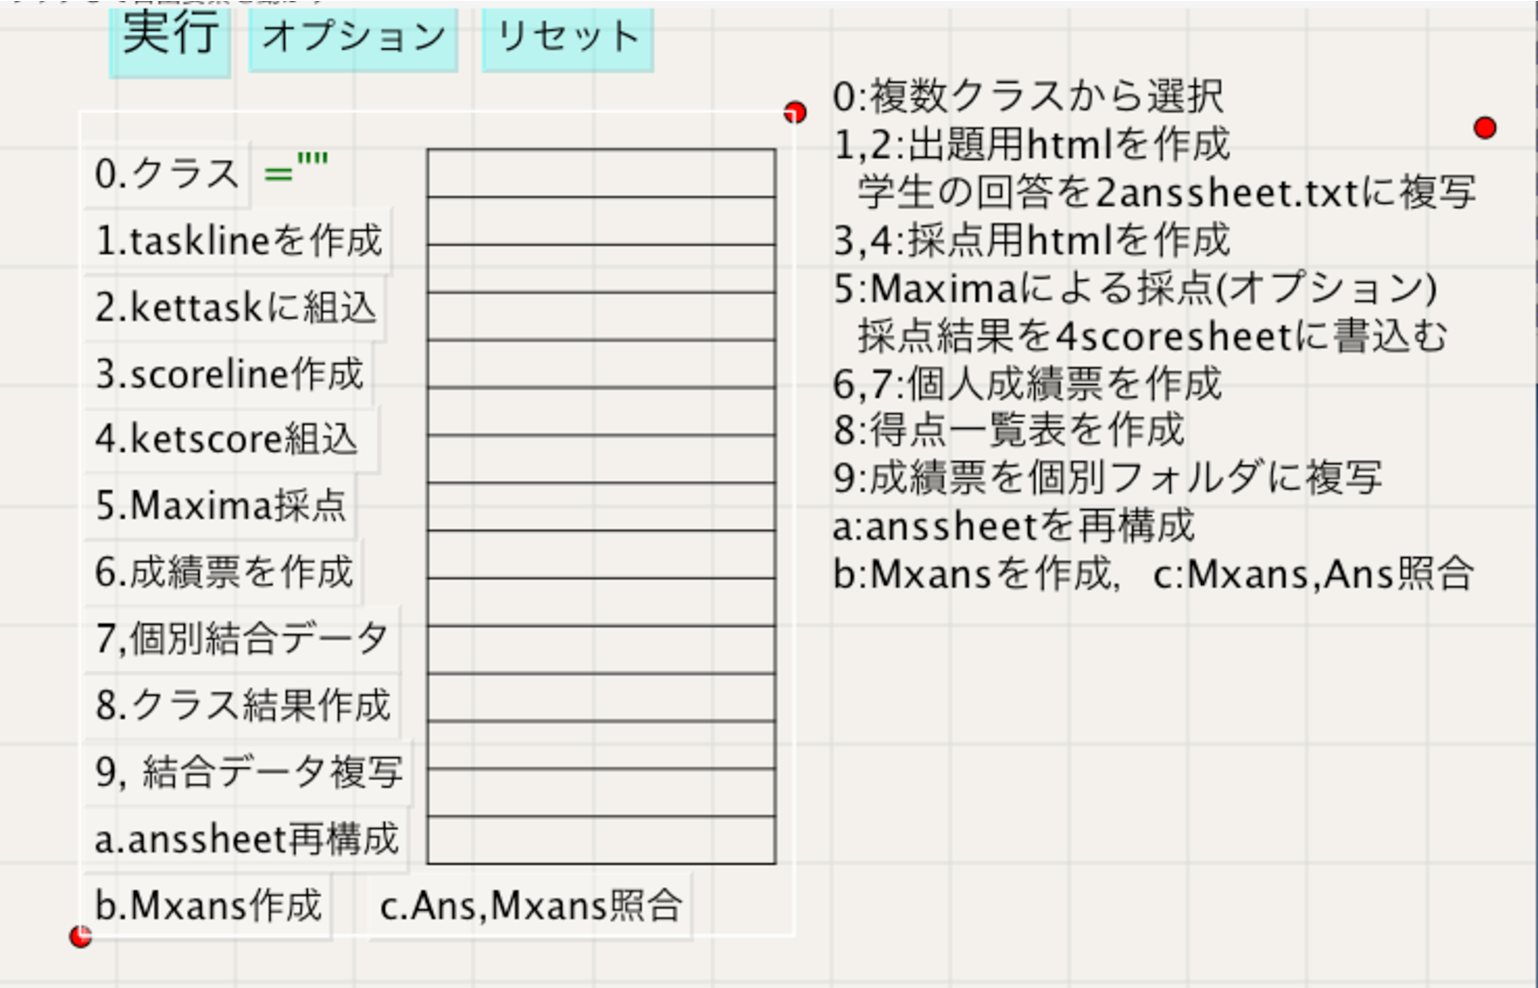
\includegraphics[bb=0.00 0.00 738.00 474.00,height=60mm]{fig/toolketmath.pdf}}
\end{layer}

{\color{red}\small

\begin{layer}{120}{0}
\end{layer}

}
%%%%%%%%%%%%

%%%%%%%%%%%%%%%%%%%%


\sameslide

\vspace*{18mm}

\slidepage
\begin{itemize}
\item
Toolketmath.cdy:KeTLMSの処理を行うツール集
\end{itemize}

\begin{layer}{120}{0}
\putnotes{72}{2}{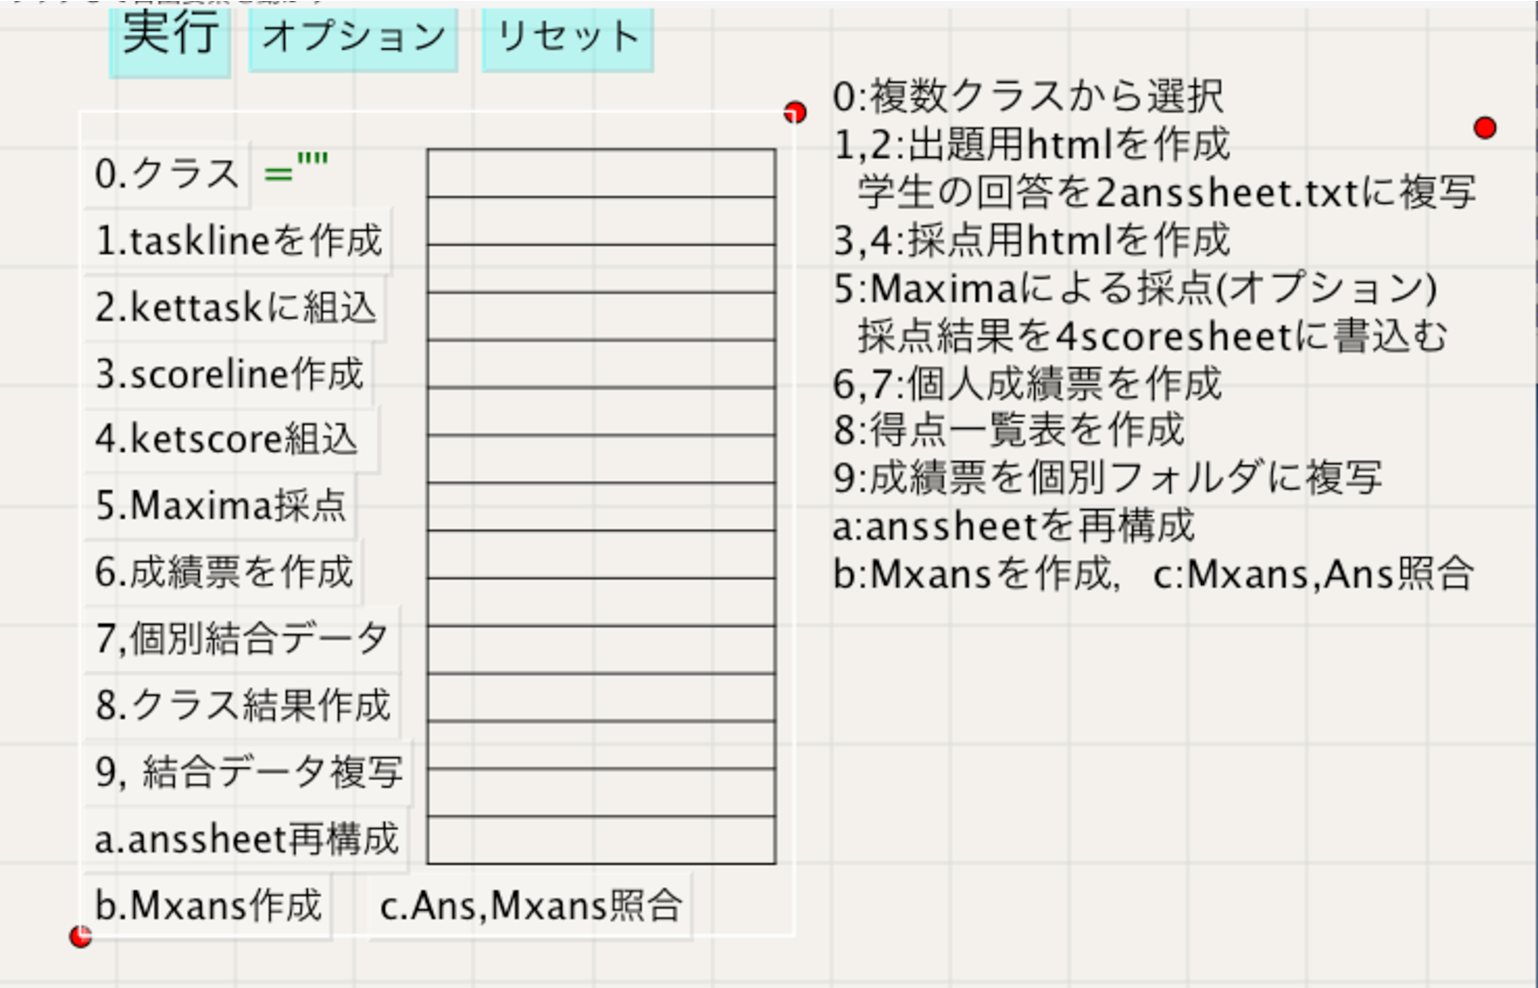
\includegraphics[bb=0.00 0.00 738.00 474.00,height=60mm]{fig/toolketmath.pdf}}
\end{layer}

{\color{red}\small

\begin{layer}{120}{0}
\putnotee{-5}{17}{問題ファイルから}
\putnotee{-5}{20.5}{ kettask作成}
\end{layer}

}

\sameslide

\vspace*{18mm}

\slidepage
\begin{itemize}
\item
Toolketmath.cdy:KeTLMSの処理を行うツール集
\end{itemize}

\begin{layer}{120}{0}
\putnotes{72}{2}{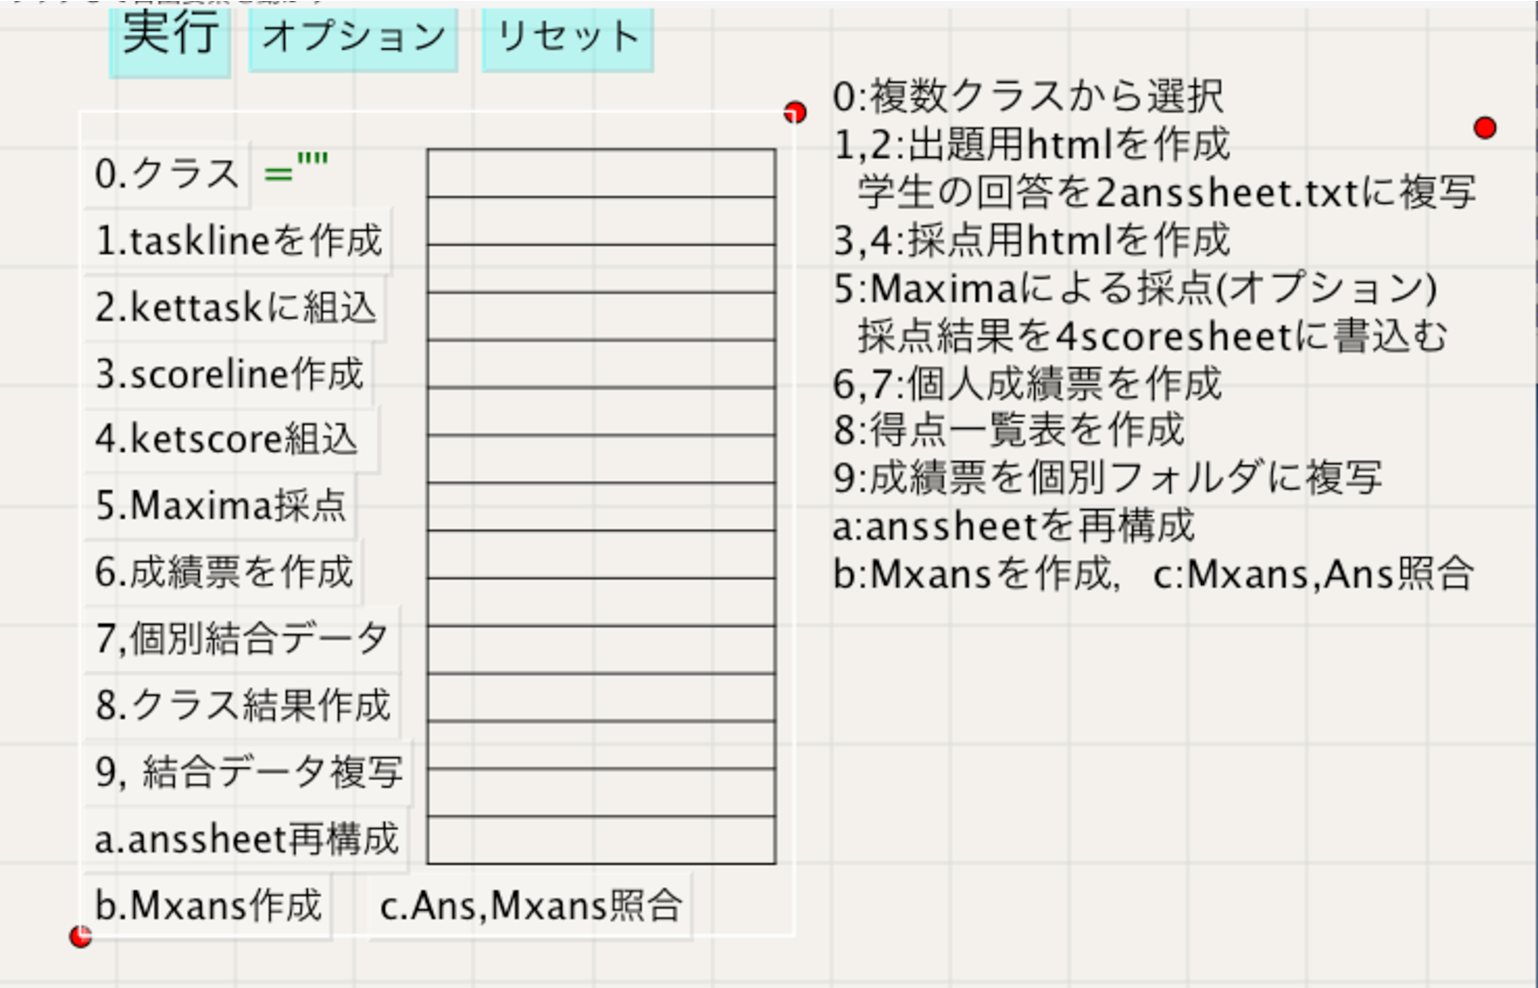
\includegraphics[bb=0.00 0.00 738.00 474.00,height=60mm]{fig/toolketmath.pdf}}
\end{layer}

{\color{red}\small

\begin{layer}{120}{0}
\putnotee{-5}{17}{問題ファイルから}
\putnotee{-5}{20.5}{ kettask作成}
\putnotee{-5}{25}{学生の回答から}
\putnotee{-5}{28.5}{ ketscore作成}
\end{layer}

}

\sameslide

\vspace*{18mm}

\slidepage
\begin{itemize}
\item
Toolketmath.cdy:KeTLMSの処理を行うツール集
\end{itemize}

\begin{layer}{120}{0}
\putnotes{72}{2}{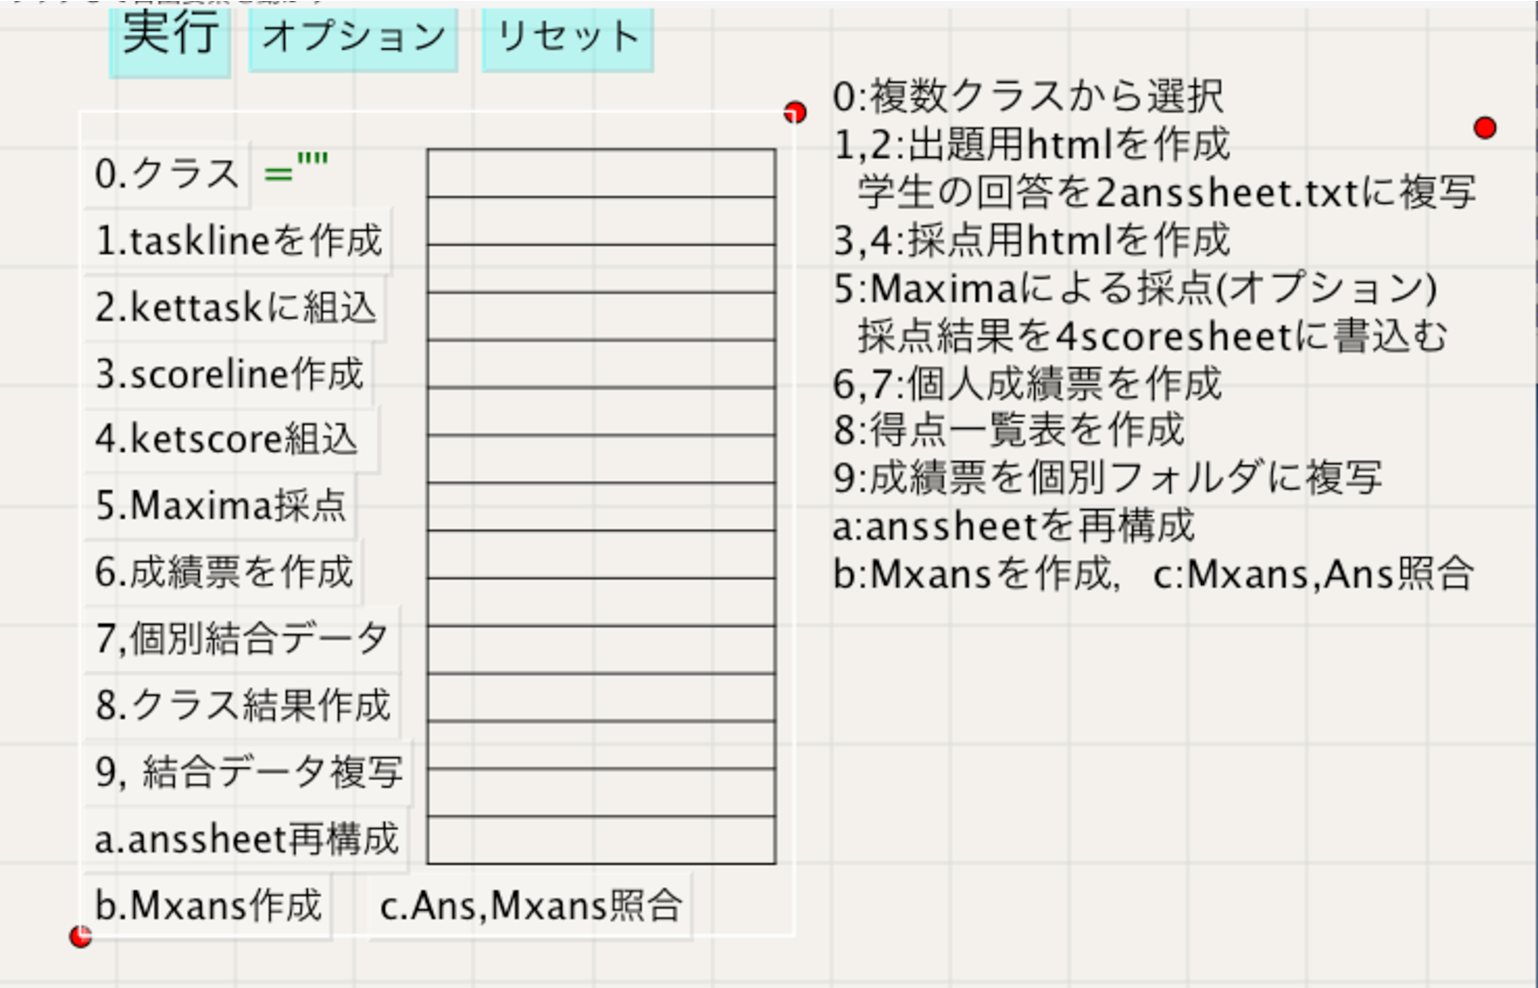
\includegraphics[bb=0.00 0.00 738.00 474.00,height=60mm]{fig/toolketmath.pdf}}
\end{layer}

{\color{red}\small

\begin{layer}{120}{0}
\putnotee{-5}{17}{問題ファイルから}
\putnotee{-5}{20.5}{ kettask作成}
\putnotee{-5}{25}{学生の回答から}
\putnotee{-5}{28.5}{ ketscore作成}
\putnotee{-5}{32}{Maximaによる採点}
\end{layer}

}

\sameslide

\vspace*{18mm}

\slidepage
\begin{itemize}
\item
Toolketmath.cdy:KeTLMSの処理を行うツール集
\end{itemize}

\begin{layer}{120}{0}
\putnotes{72}{2}{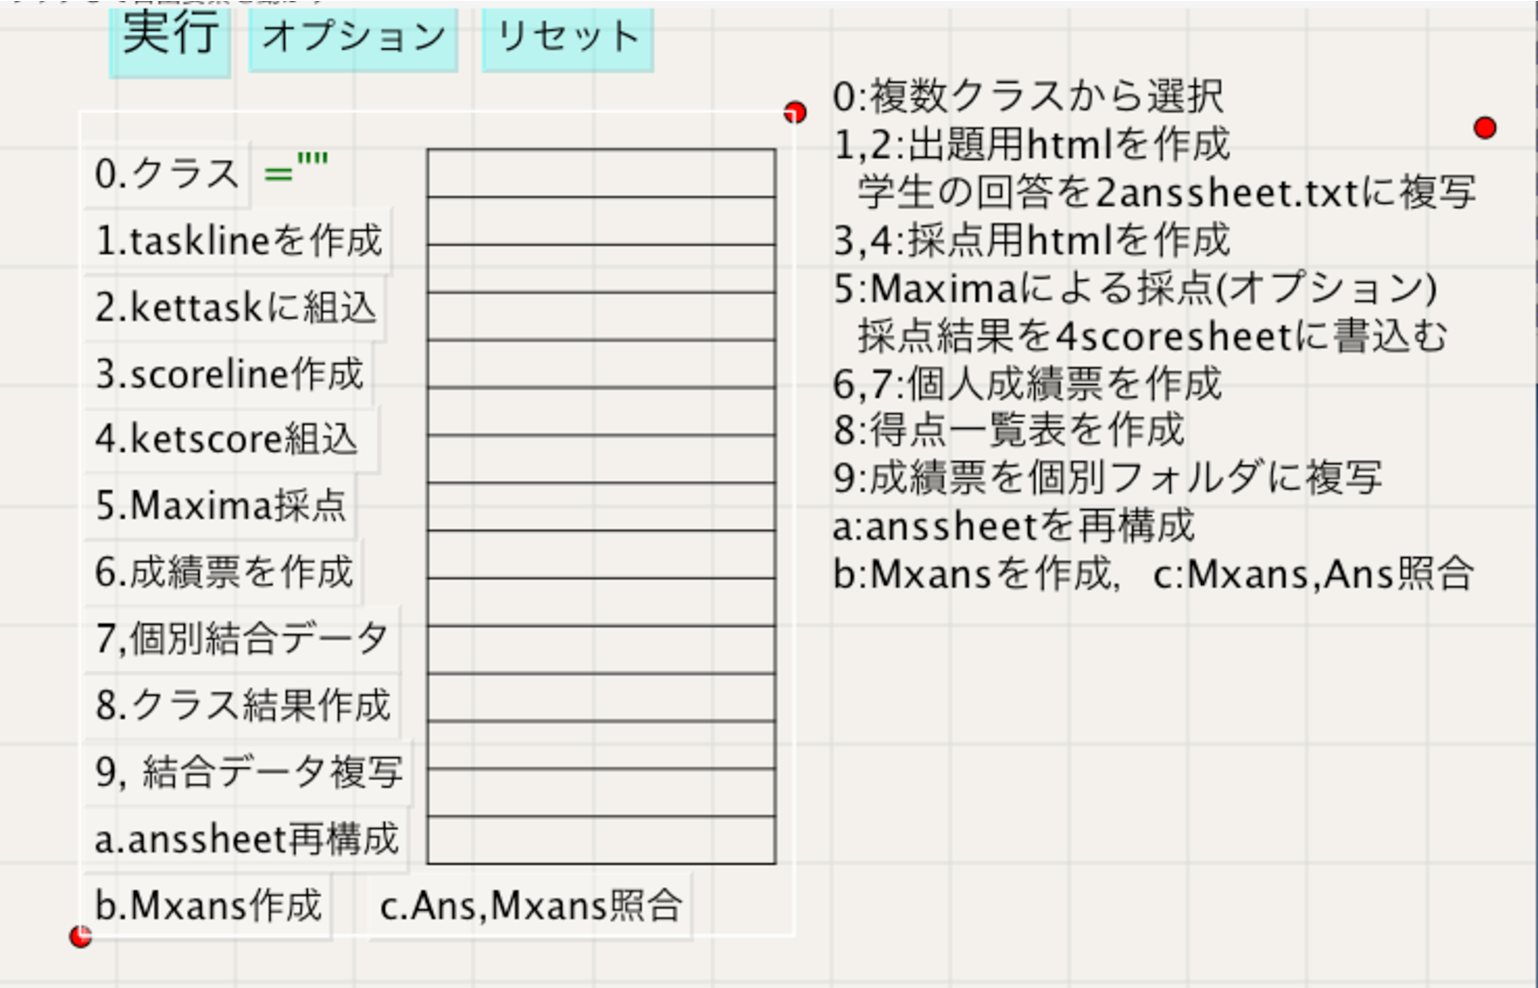
\includegraphics[bb=0.00 0.00 738.00 474.00,height=60mm]{fig/toolketmath.pdf}}
\end{layer}

{\color{red}\small

\begin{layer}{120}{0}
\putnotee{-5}{17}{問題ファイルから}
\putnotee{-5}{20.5}{ kettask作成}
\putnotee{-5}{25}{学生の回答から}
\putnotee{-5}{28.5}{ ketscore作成}
\putnotee{-5}{32}{Maximaによる採点}
\putnotee{-5}{36.5}{学生別課題別成績票}
\end{layer}

}

\sameslide

\vspace*{18mm}

\slidepage
\begin{itemize}
\item
Toolketmath.cdy:KeTLMSの処理を行うツール集
\end{itemize}

\begin{layer}{120}{0}
\putnotes{72}{2}{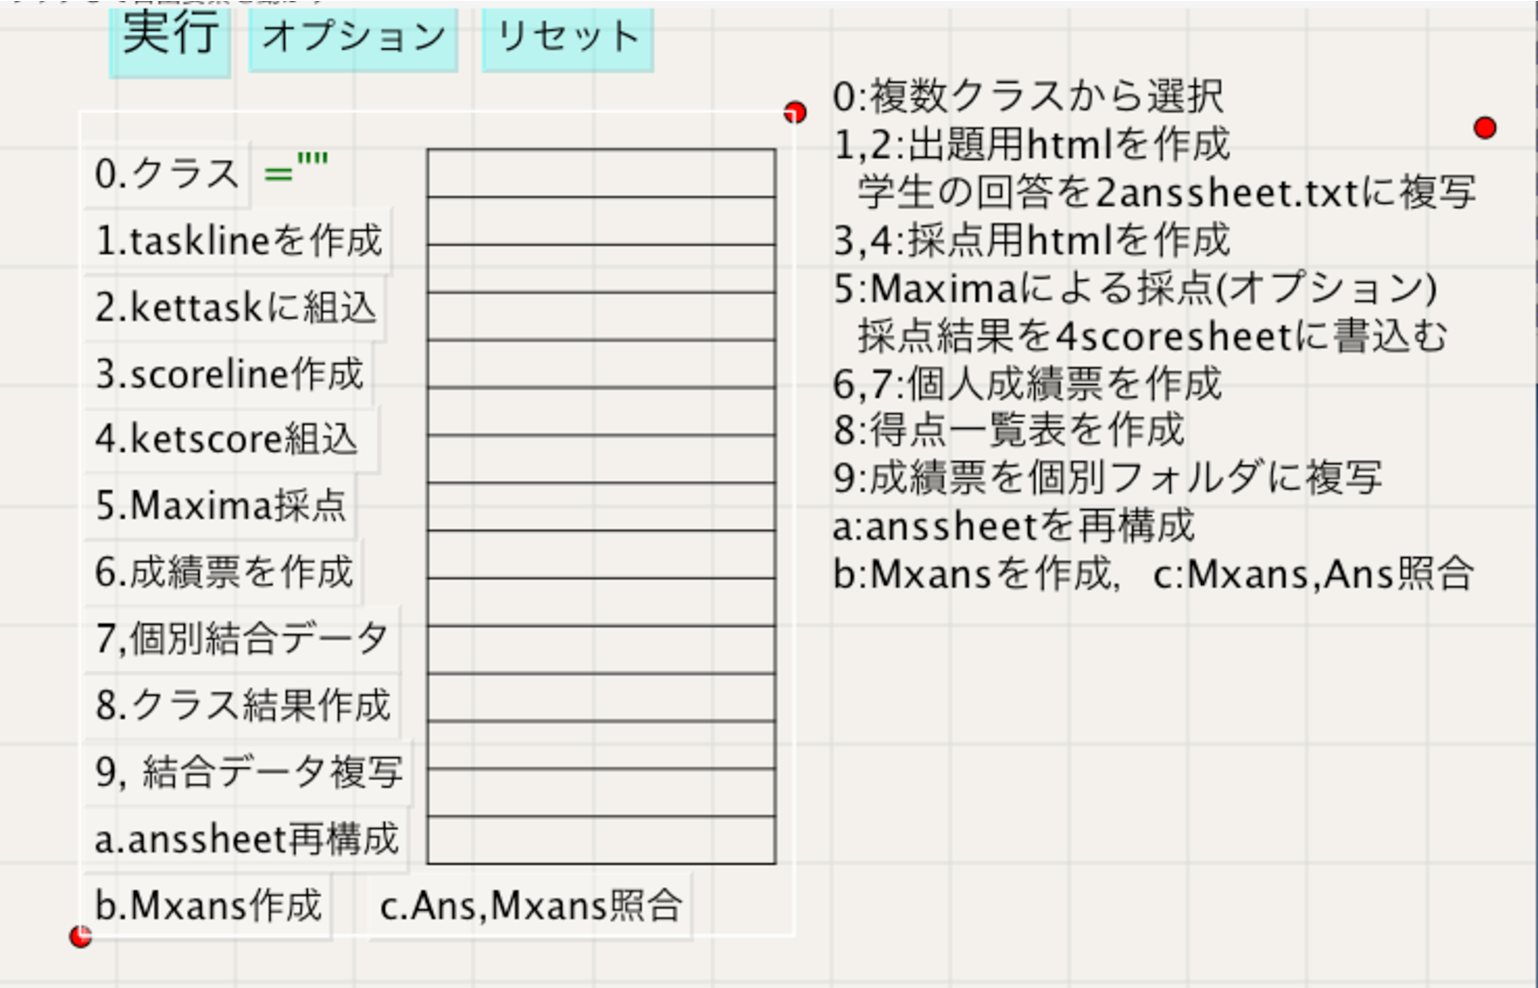
\includegraphics[bb=0.00 0.00 738.00 474.00,height=60mm]{fig/toolketmath.pdf}}
\end{layer}

{\color{red}\small

\begin{layer}{120}{0}
\putnotee{-5}{17}{問題ファイルから}
\putnotee{-5}{20.5}{ kettask作成}
\putnotee{-5}{25}{学生の回答から}
\putnotee{-5}{28.5}{ ketscore作成}
\putnotee{-5}{32}{Maximaによる採点}
\putnotee{-5}{36.5}{学生別課題別成績票}
\putnotee{-5}{41}{学生別成績票}
\end{layer}

}

\sameslide

\vspace*{18mm}

\slidepage
\begin{itemize}
\item
Toolketmath.cdy:KeTLMSの処理を行うツール集
\end{itemize}

\begin{layer}{120}{0}
\putnotes{72}{2}{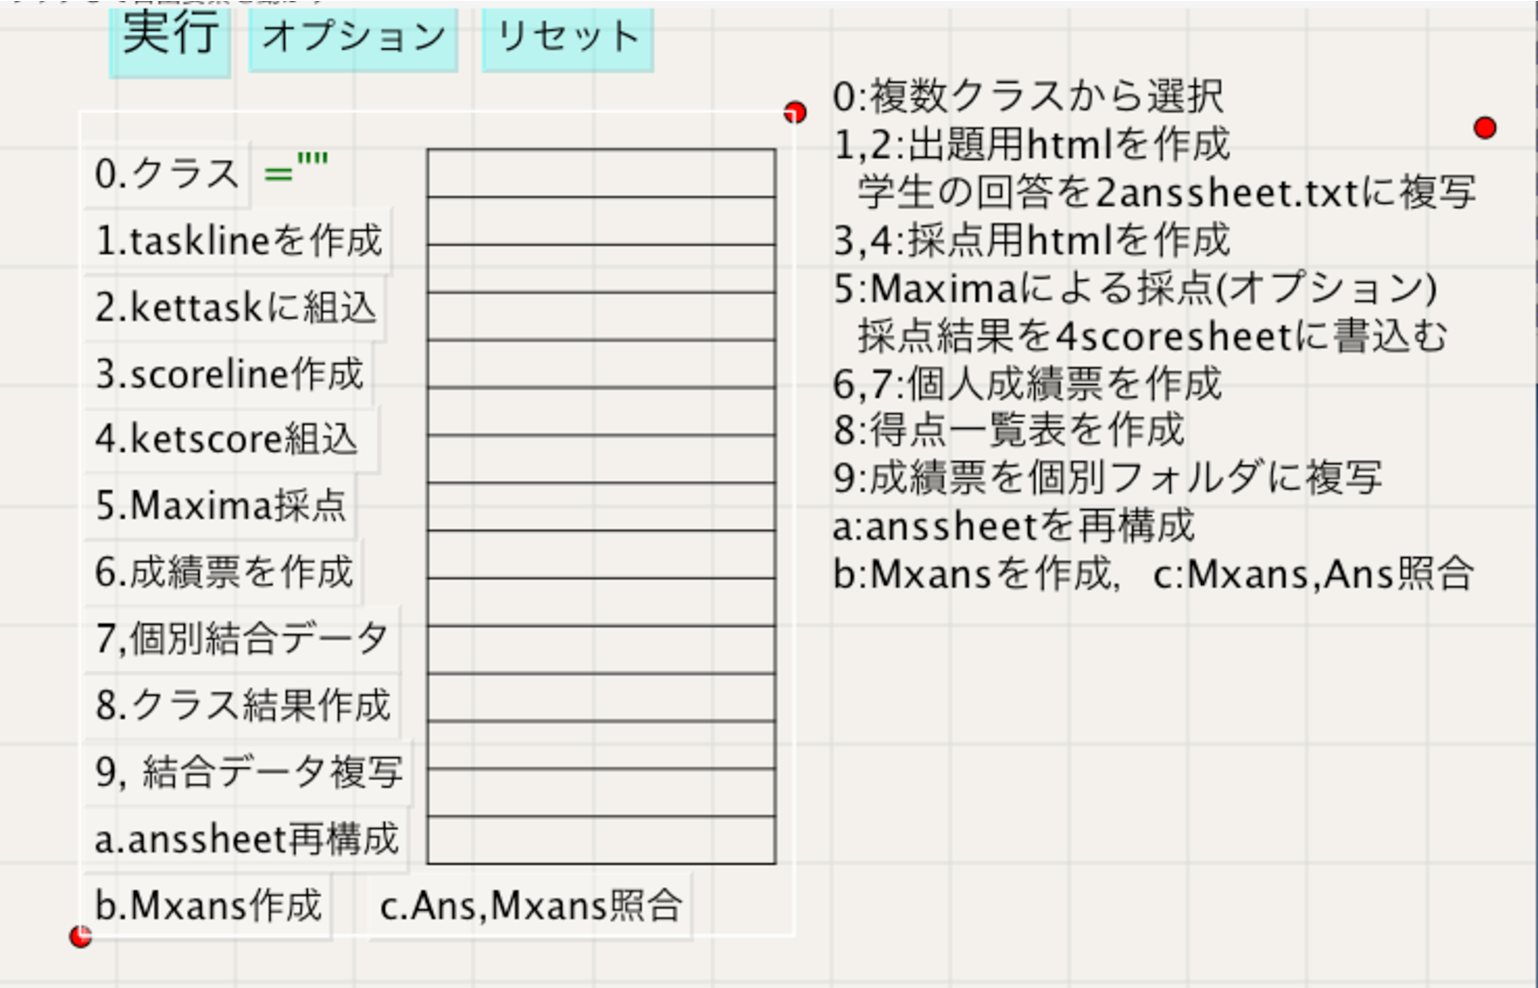
\includegraphics[bb=0.00 0.00 738.00 474.00,height=60mm]{fig/toolketmath.pdf}}
\end{layer}

{\color{red}\small

\begin{layer}{120}{0}
\putnotee{-5}{17}{問題ファイルから}
\putnotee{-5}{20.5}{ kettask作成}
\putnotee{-5}{25}{学生の回答から}
\putnotee{-5}{28.5}{ ketscore作成}
\putnotee{-5}{32}{Maximaによる採点}
\putnotee{-5}{36.5}{学生別課題別成績票}
\putnotee{-5}{41}{学生別成績票}
\putnotee{-5}{45}{クラス成績一覧表}
\end{layer}

}

\sameslide

\vspace*{18mm}

\slidepage
\begin{itemize}
\item
Toolketmath.cdy:KeTLMSの処理を行うツール集
\end{itemize}

\begin{layer}{120}{0}
\putnotes{72}{2}{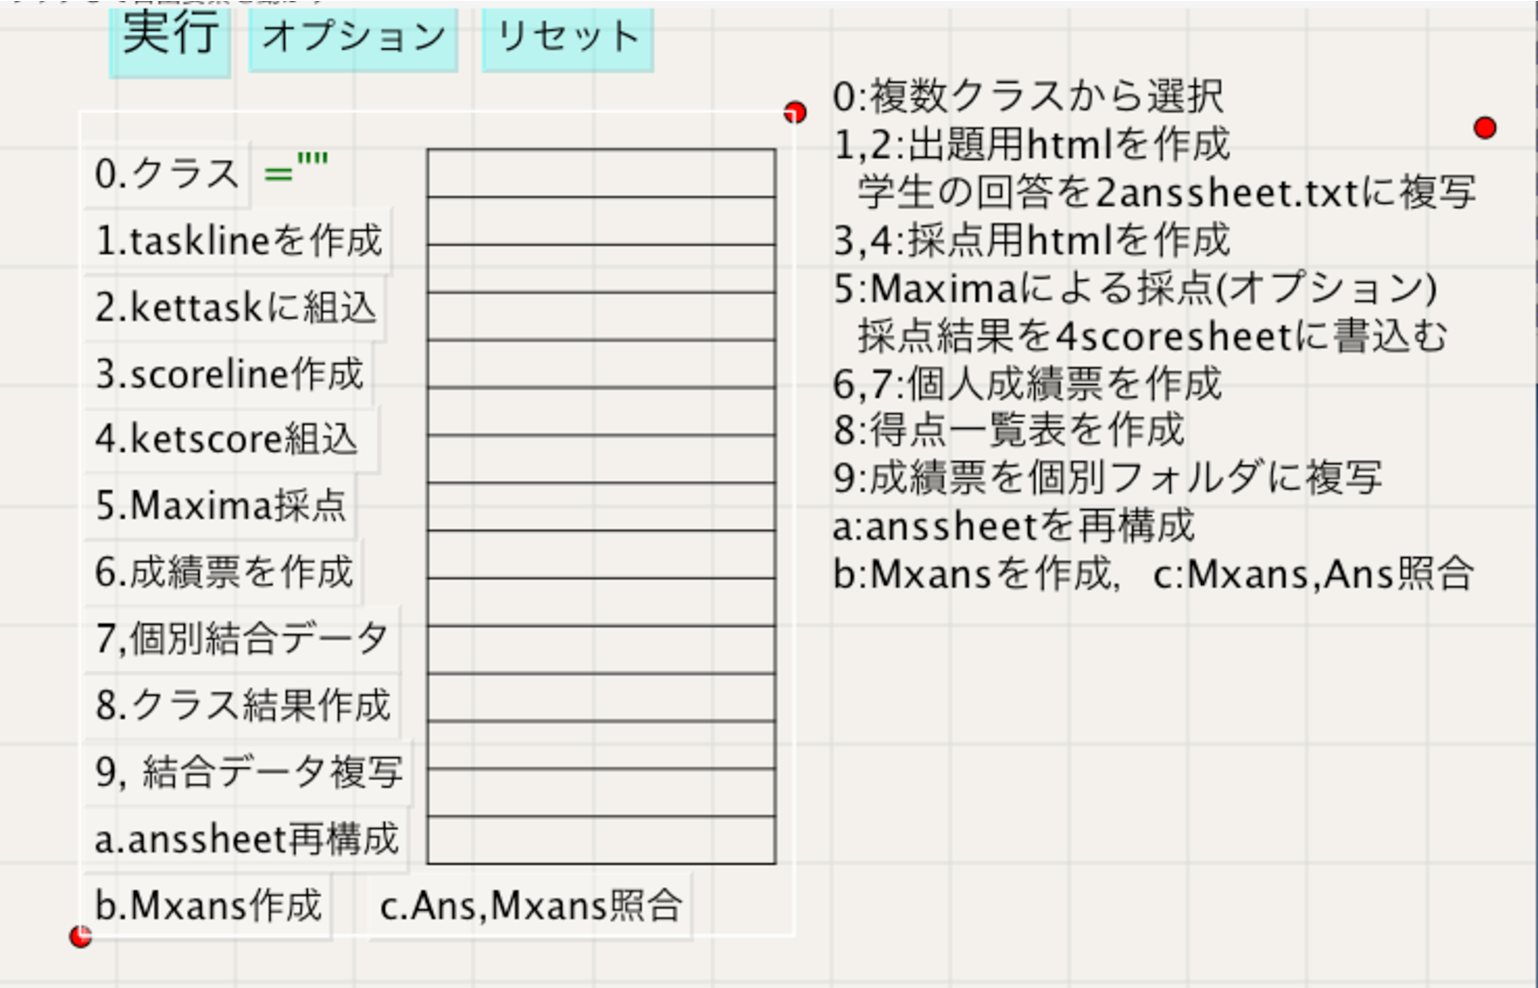
\includegraphics[bb=0.00 0.00 738.00 474.00,height=60mm]{fig/toolketmath.pdf}}
\end{layer}

{\color{red}\small

\begin{layer}{120}{0}
\putnotee{-5}{17}{問題ファイルから}
\putnotee{-5}{20.5}{ kettask作成}
\putnotee{-5}{25}{学生の回答から}
\putnotee{-5}{28.5}{ ketscore作成}
\putnotee{-5}{32}{Maximaによる採点}
\putnotee{-5}{36.5}{学生別課題別成績票}
\putnotee{-5}{41}{学生別成績票}
\putnotee{-5}{45}{クラス成績一覧表}
\putnotee{-5}{49}{成績票を配付}
\end{layer}

}

\sameslide

\vspace*{18mm}

\slidepage
\begin{itemize}
\item
Toolketmath.cdy:KeTLMSの処理を行うツール集
\end{itemize}

\begin{layer}{120}{0}
\putnotes{72}{2}{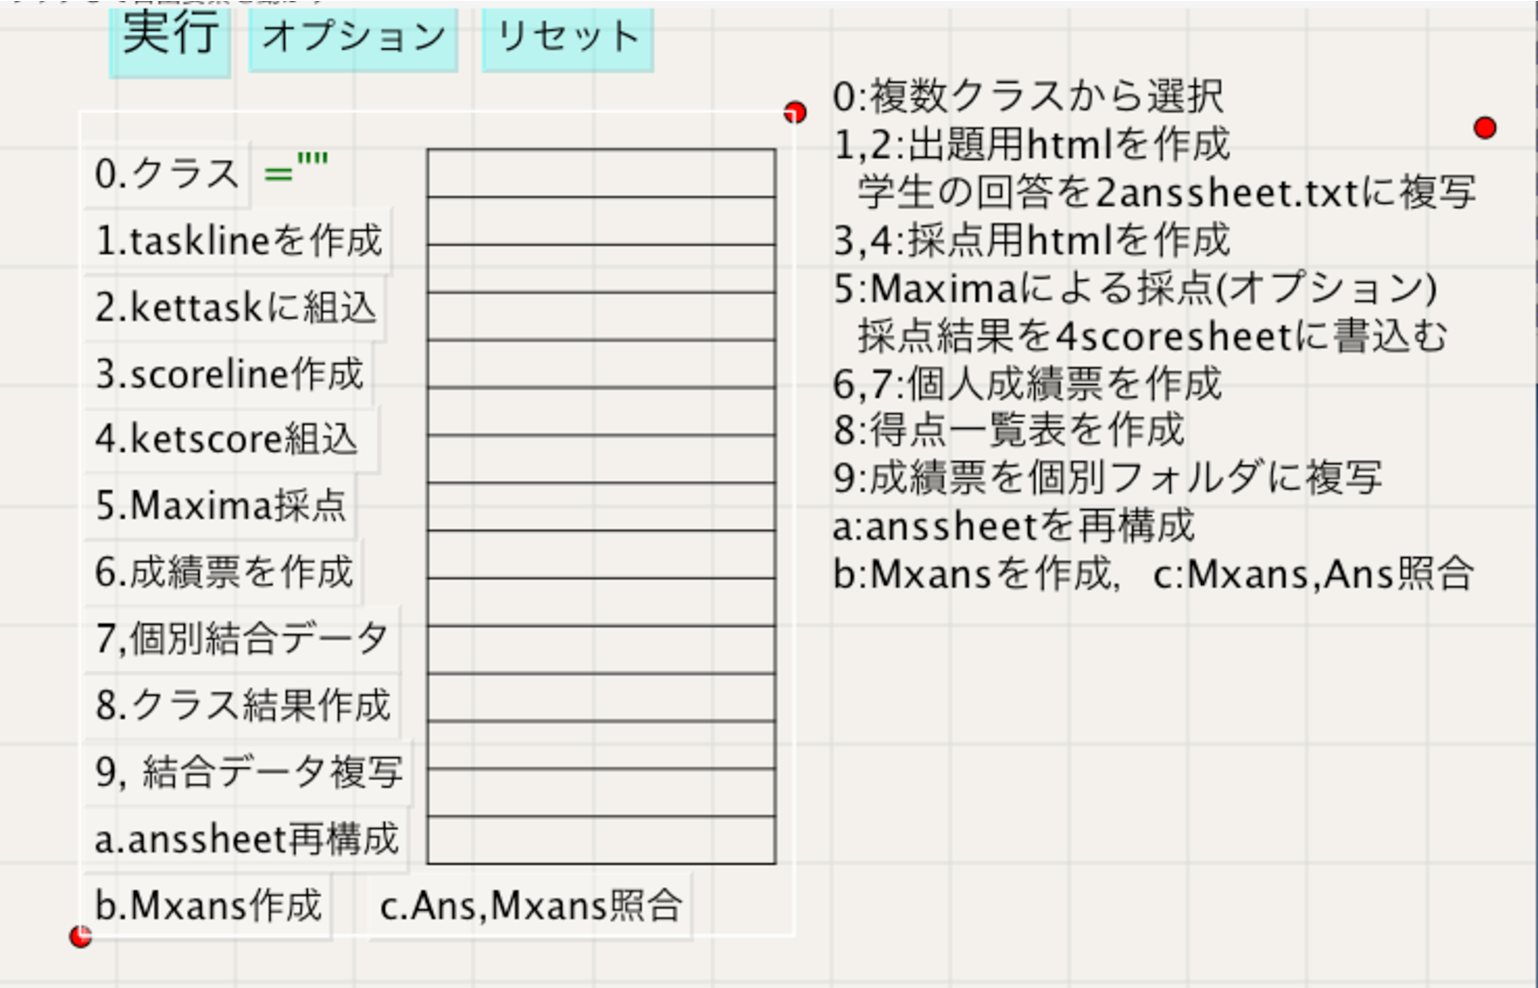
\includegraphics[bb=0.00 0.00 738.00 474.00,height=60mm]{fig/toolketmath.pdf}}
\end{layer}

{\color{red}\small

\begin{layer}{120}{0}
\putnotee{-5}{17}{問題ファイルから}
\putnotee{-5}{20.5}{ kettask作成}
\putnotee{-5}{25}{学生の回答から}
\putnotee{-5}{28.5}{ ketscore作成}
\putnotee{-5}{32}{Maximaによる採点}
\putnotee{-5}{36.5}{学生別課題別成績票}
\putnotee{-5}{41}{学生別成績票}
\putnotee{-5}{45}{クラス成績一覧表}
\putnotee{-5}{49}{成績票を配付}
\putnotee{-5}{52.5}{ Dropboxの}
\putnotee{-5}{56}{ リンクを通知}
\end{layer}

}

\newslide{従来の授業との比較}

\vspace*{18mm}

\slidepage
\begin{itemize}
\item
テキストのやり取りは処理が楽でトラブルが少ない\\
\end{itemize}

\sameslide

\vspace*{18mm}

\slidepage
\begin{itemize}
\item
テキストのやり取りは処理が楽でトラブルが少ない\\
 $\Longrightarrow$ {\color{red}成績処理の労力を軽減}
\end{itemize}

\sameslide

\vspace*{18mm}

\slidepage
\begin{itemize}
\item
テキストのやり取りは処理が楽でトラブルが少ない\\
 $\Longrightarrow$ {\color{red}成績処理の労力を軽減}
\item
授業中に複数回できる(授業のリズム,理解度チェック)\\
 昨年の実績 5−8回/1授業
\end{itemize}

\sameslide

\vspace*{18mm}

\slidepage
\begin{itemize}
\item
テキストのやり取りは処理が楽でトラブルが少ない\\
 $\Longrightarrow$ {\color{red}成績処理の労力を軽減}
\item
授業中に複数回できる(授業のリズム,理解度チェック)\\
 昨年の実績 5−8回/1授業
\item
講義をしながら採点処理するのはまだ\\
\end{itemize}

\sameslide

\vspace*{18mm}

\slidepage
\begin{itemize}
\item
テキストのやり取りは処理が楽でトラブルが少ない\\
 $\Longrightarrow$ {\color{red}成績処理の労力を軽減}
\item
授業中に複数回できる(授業のリズム,理解度チェック)\\
 昨年の実績 5−8回/1授業
\item
講義をしながら採点処理するのはまだ\\
 $\Longrightarrow$ 今後の課題\\ 
   $\left\{\begin{array}{l}
    \mbox{Maxima採点のエラーをなくす}\\
    \mbox{一連の処理を自動化(特に採点)}
    \end{array}\right.$
\end{itemize}
\label{pageend}\mbox{}

\end{document}
